%%%%%%%%%%%%%%%%%%%%%%%%%%%%%%%%%%%%%%%%%%%%%%%%%%%%%%%%%%%%%%%%%%%%%%%%%%%
%% Copyright (C) 2012 Minh Van Nguyen <mvngu.name@gmail.com>
%%%%%%%%%%%%%%%%%%%%%%%%%%%%%%%%%%%%%%%%%%%%%%%%%%%%%%%%%%%%%%%%%%%%%%%%%%%

\documentclass{article}

\usepackage{subfigure}
\usepackage{tikz}
\usetikzlibrary{external}
\usetikzlibrary{fit}
\usetikzlibrary{shapes}
\tikzexternalize{match}

\begin{document}

\begin{figure}
\subfigure[]{
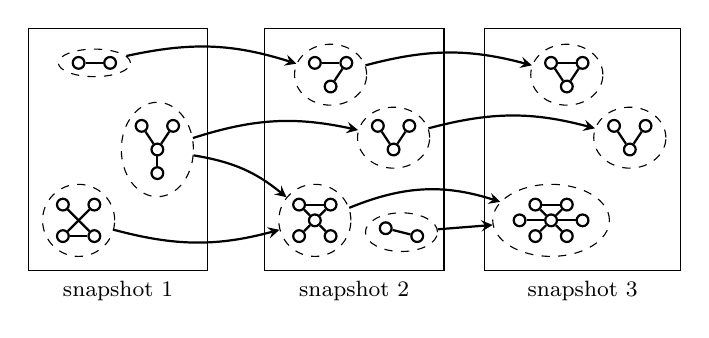
\begin{tikzpicture}
[lineDecorate/.style={-,thick},%
  nodeDecorate/.style={shape=circle,inner sep=1.5pt,draw,thick},
  every fit/.style={ellipse,draw,dashed,inner sep=1pt}]
%%
%%%%%%%%%%%%%%%%%%%%%%%%%%%%%%%%%%%%%%%%%%%%%%%%%%%%%%%%%%%%%%%%%%%%%%%%%%%
%%
%% snapshot 1
%% nodes or vertices
\foreach \nodename/\x/\y in {
  0/0/0, 1/0.4/0, 2/0.4/0.4, 3/0/0.4,
  4/1/1.4, 5/1.4/1.4, 6/1.2/0.8, 7/1.2/1.1,
  8/0.2/2.2, 9/0.6/2.2}
{
  \node (\nodename) at (\x,\y) [nodeDecorate] {};
}
%% edges or lines
\path
\foreach \startnode/\endnode in {
  0/1, 0/2, 1/3,
  4/7, 5/7, 6/7,
  8/9}
{
  (\startnode) edge[lineDecorate] node {} (\endnode)
};
%% encircle each community
\node (c0) [fit=(0) (1) (2) (3)] {};
\node (c1) [fit=(4) (5) (6) (7)] {};
\node (c2) [fit=(8) (9)] {};
\node[fit=(0) (1) (2) (3) (4) (5) (6) (7) (8) (9),%%
  rectangle,inner sep=10pt,draw,solid,%%
  label=below:{\footnotesize snapshot~1}] {};
%%
%%%%%%%%%%%%%%%%%%%%%%%%%%%%%%%%%%%%%%%%%%%%%%%%%%%%%%%%%%%%%%%%%%%%%%%%%%%
%%
%% snapshot 2
%% nodes or vertices
\foreach \nodename/\x/\y in {
  20/3/0, 21/3.4/0, 22/3.4/0.4, 23/3/0.4, 211/3.2/0.2,
  24/4/1.4, 25/4.4/1.4, 27/4.2/1.1,
  28/3.2/2.2, 29/3.6/2.2, 210/3.4/1.9,
  212/4.1/0.1, 213/4.5/0.0}
{
  \node (\nodename) at (\x,\y) [nodeDecorate] {};
}
%% edges or lines
\path
\foreach \startnode/\endnode in {
  20/211, 21/211, 22/23, 23/211, 22/211,
  24/27, 25/27,
  28/29, 29/210,
  212/213}
{
  (\startnode) edge[lineDecorate] node {} (\endnode)
};
%% encircle each community
\node (c3) [fit=(20) (21) (22) (23)] {};
\node (c4) [fit=(24) (25) (27)] {};
\node (c5) [fit=(28) (29) (210)] {};
\node (c6) [fit=(212) (213)] {};
\node[fit=(20) (21) (22) (23) (24) (25) (27) (28) (29) (210),%%
  rectangle,inner sep=10pt,draw,solid,%%
  label=below:{\footnotesize snapshot~2}] {};
%%
%%%%%%%%%%%%%%%%%%%%%%%%%%%%%%%%%%%%%%%%%%%%%%%%%%%%%%%%%%%%%%%%%%%%%%%%%%%
%%
%% snapshot 3
%% nodes or vertices
\foreach \nodename/\x/\y in {
  30/6/0, 31/6.4/0, 32/6.4/0.4, 33/6/0.4, 311/6.2/0.2, 314/5.8/0.2,
  315/6.6/0.2,
  %%
  34/7/1.4, 35/7.4/1.4, 37/7.2/1.1,
  38/6.2/2.2, 39/6.6/2.2, 310/6.4/1.9}
{
  \node (\nodename) at (\x,\y) [nodeDecorate] {};
}
%% edges or lines
\path
\foreach \startnode/\endnode in {
  30/311, 31/311, 32/33, 33/311, 32/311, 311/314, 311/315,
  34/37, 35/37,
  38/310, 39/310, 38/39}
{
  (\startnode) edge[lineDecorate] node {} (\endnode)
};
%% encircle each community
\node (c7) [fit=(30) (31) (32) (33) (311) (314) (315)] {};
\node (c8) [fit=(34) (35) (37)] {};
\node (c9) [fit=(38) (39) (310)] {};
\node[fit=(30) (31) (32) (33) (34) (35) (37) (38) (39) (310) (314),%%
  rectangle,inner sep=10pt,draw,solid,%%
  label=below:{\footnotesize snapshot~3}] {};
%%
%%%%%%%%%%%%%%%%%%%%%%%%%%%%%%%%%%%%%%%%%%%%%%%%%%%%%%%%%%%%%%%%%%%%%%%%%%%
%%
%% continuity across snapshots
\path
(c0) edge[thick,bend right=15,->,>=stealth] node {} (c3)
(c1) edge[thick,bend left=15,->,>=stealth] node {} (c3)
(c1) edge[thick,bend left=15,->,>=stealth] node {} (c4)
(c2) edge[thick,bend left=15,->,>=stealth] node {} (c5)
(c3) edge[thick,bend left=20,->,>=stealth] node {} (c7)
(c4) edge[thick,bend left=15,->,>=stealth] node {} (c8)
(c5) edge[thick,bend left=15,->,>=stealth] node {} (c9)
(c6) edge[thick,->,>=stealth] node {} (c7);
\end{tikzpicture}
}
\end{figure}

\end{document}
